\chapter{Реализация и экспериментальная проверка серверного контура обнаружения дефектов 3D-печати}

\section{Формирование набора данных, аннотирование и аугментация изображений}

Качество обнаружения дефектов в процессе~3D-печати напрямую зависит от качества исходного набора данных. Поэтому подготовка датасета выделена в отдельный инженерный этап с фиксированными правилами отбора, аннотирования и проверки разметки.

В данной работе датасет формируется преимущественно на основе собственных экспериментальных печатей: не менее 80~\% кадров собираются на разработанной установке в реальных условиях эксплуатации. До 20~\% изображений добавляются из открытых источников для расширения вариативности сцен и повышения устойчивости модели. Такой баланс сохраняет привязку к целевой конфигурации принтера и снижает риск переобучения на узкий набор условий.

Сбор основной части данных автоматизирован на уровне рабочего контура печати. После запуска задания макрос \texttt{START\_PRINT} вызывает \texttt{\_TREED\_CAM\_START}, который через Moonraker (API-сервис обмена командами и телеметрией) запускает \texttt{treed\_cam\_session\_start}. Скрипт \texttt{session\_start.sh} создает каталог сессии в \texttt{/home/pi/treed/cam/prints}, записывает путь в маркерный файл \texttt{/tmp/treed\_cam\_session\_dir} и сохраняет стартовый кадр.

Дальнейшая съемка выполняется периодически в процессе печати. Макрос \texttt{\_TREED\_CAM\_TICK} вызывает \texttt{treed\_cam\_snapshot}, а \texttt{snapshot.sh} добавляет кадры в каталог активной сессии. Интервал задается параметром \texttt{snapshot\_interval} в \texttt{\_TREED\_PRINT\_DEFAULTS}; в базовой конфигурации используется \(120~\text{с}\) с нижним ограничением \(10~\text{с}\). После завершения задания макрос \texttt{END\_PRINT} выполняет \texttt{\_TREED\_CAM\_STOP} и закрывает сессию.

При отборе изображений исключаются дубли, кадры с критически низкой резкостью и примеры, где зона печати не позволяет однозначно интерпретировать состояние процесса. В набор включаются кадры с дефектами и кадры штатной печати без отклонений.

Аннотирование выполняется в Roboflow в формате ограничивающих прямоугольников. Для каждой аннотации контролируются точность границ, отсутствие дублирующих рамок и соответствие фактической области дефекта.

Критичными ошибками считаются завышенные ограничивающие рамки и перекрытие нескольких рамок на одном дефекте. На рисунках~\ref{fig:big} и~\ref{fig:Granitsi} показаны эти случаи.

На рисунке~\ref{fig:big} ограничивающая рамка существенно превышает реальную область дефекта. В рамку попадает значительная часть фона. Это искажает геометрию объекта и ухудшает обучение модели.

На рисунке~\ref{fig:Granitsi} несколько рамок размечают один и тот же дефект. Такая разметка создает дубли и формирует неоднозначные обучающие примеры. При накоплении подобных ошибок снижается устойчивость модели на проверочных данных.

\begin{figure}[h!]
  \begin{minipage}[b]{0.45\hsize}
    \centering
    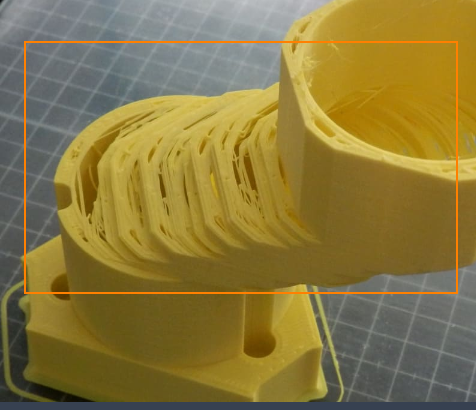
\includegraphics[width=\hsize]{fig/big.png}
    \caption{Слишком большие границы дефекта}
    \label{fig:big}
  \end{minipage}
  \hfill
  \begin{minipage}[b]{0.45\hsize}
    \centering
    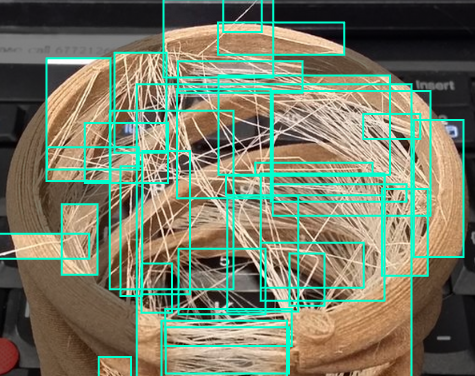
\includegraphics[width=\hsize]{fig/Granitsi.png}
    \caption{Границы дефектов перекрывают друг друга}
    \label{fig:Granitsi}
  \end{minipage}
\end{figure}

Качество разметки оценивается с учетом метрики Intersection over Union, которая отражает степень совпадения предсказанной и эталонной области. Неточные границы напрямую снижают значение этой метрики и ухудшают итоговое качество обнаружения. Поэтому автоматическая разметка используется только как вспомогательный шаг, а финальная валидация выполняется вручную.

После формирования исходного набора применяется аугментация изображений для повышения устойчивости к изменениям условий съемки. Используются преобразования яркости, контраста, умеренный шум и небольшие геометрические изменения, которые не разрушают структуру дефекта. Далее датасет разделяется на обучающую, валидационную и тестовую части с контролем представленности целевых дефектов.

В результате формируется датасет, ориентированный на реальные условия работы разработанного комплекса и пригодный для обучения серверной модели обнаружения дефектов. Принятые правила разметки и контроля качества снижают влияние шумовых факторов и повышают воспроизводимость экспериментов. На основе этого набора данных в следующем разделе рассматривается реализация серверного контура обработки визуальных данных.


\section{Реализация серверного контура обработки визуальных данных}

\section{Интеграция серверного анализа с контуром управления 3D-принтером}

\section{Результаты экспериментальных запусков, ограничения и направления развития}
